\documentclass[10pt,twocolumn]{article}

\usepackage[a4paper, top=30mm, bottom=20mm, left=10mm, right=10mm]{geometry}
\usepackage[hangul]{kotex}
\newcommand{\titleko}{람다 계산법을 응용한 자연 연역 체계의 전산화에 관한 연구}
\newcommand{\titleen}{Computerizing natural deduction using lambda calculus}
\newcommand{\authorname}{이상길}
\newcommand{\getkeywords}{수학기초론, 람다 계산법, 자연 연역 체계}
\usepackage[pdfencoding=unicode,
	pdfauthor={\authorname},
	pdftitle={\titleko},
	pdfkeywords={\getkeywords},
	bookmarks]{hyperref}
\usepackage{amsmath, amscd, amsthm, amssymb, amsfonts, mathrsfs, mathtools, mathalfa}
\usepackage{abstract}
\usepackage[sans]{dsfont}
\usepackage{latexsym}
\usepackage{enumitem}
\usepackage{color}
\usepackage{url}
\usepackage{graphicx}
\graphicspath{{./images/}}
\usepackage{multirow}
\usepackage{float}
\usepackage{listings}
\usepackage[square,numbers]{natbib}
\bibliographystyle{ieeetr}
\usepackage{caption}
\captionsetup[table]{skip=.5em}
\usepackage{fitch}
\usepackage{bm}
\usepackage{adjustbox}

\definecolor{javared}{rgb}{0.6,0,0}
\definecolor{javapurple}{rgb}{0.5,0,0.35}

\lstdefinelanguage{mom}{
	keywords={type,axiom,theorem},
	sensitive=true,
	keywordstyle=\color{javapurple}\ttfamily,
	morecomment=[s][\color{javared}]{<}{>},
}

\lstset{
	language=mom,
	basicstyle=\small\ttfamily,
	numberstyle=\small\ttfamily,
	tabsize=4,
	numbers=left,
	xleftmargin=.7cm
}

\theoremstyle{definition}
\newtheorem{theorem}{정리}
\newtheorem{definition}[theorem]{정의}
\newtheorem{example}[theorem]{예시}

\newcommand{\N}{\mathbb{N}}
\newcommand{\Z}{\mathbb{Z}}
\newcommand{\Q}{\mathbb{Q}}
\newcommand{\R}{\mathbb{R}}

\newcommand{\sinc}{\operatorname{sinc}}
\newcommand{\dom}{\operatorname{dom}}
\newcommand{\im}{\operatorname{im}}
\newcommand{\ord}{\operatorname{ord}}
\newcommand{\Prop}{\mathsf{Prop}}
\newcommand{\Cls}{\mathsf{Cls}}
\newcommand{\Predicate}{\mathsf{Predicate}}
\newcommand{\leqnormal}{\mathrel{\unlhd}}
\newcommand{\ltnormal}{\mathrel{\lhd}}

\newcommand{\lch}{\bm\lambda_\to^{\text{Ch}}}
\newcommand{\lchh}{\bm\lambda_{\to,\vdash}^{\text{Ch}}}
\newcommand{\Lch}{\Lambda_\to^{\text{Ch}}}
\newcommand{\Lchh}{\Lambda_{\to,\vdash}^{\text{Ch}}}

\newcommand{\fv}{\mathbf{FV}}
\newcommand{\bv}{\mathbf{BV}}

% \renewcommand{\abstractname}{초 록}
\renewcommand{\refname}{참고문헌}
\kscntformat{section}{}{}

\title{\titleko\\[1ex]\large\titleen}
\author{\authorname\thanks{\href{mailto:ossia@korea.ac.kr}{\texttt{ossia@korea.ac.kr}}}}
\date{}

\begin{document}

\twocolumn[
\begin{@twocolumnfalse}
	\maketitle
	\begin{abstract}
		\centering\begin{minipage}{\dimexpr\paperwidth-8cm}
			\noindent 대충 요약
			
			\smallskip\noindent {\bf 주제어}: \getkeywords
		\end{minipage}
	\end{abstract}\vspace{2em}
\end{@twocolumnfalse}
]

\saythanks

\section{서론}

형식 체계를 전산화하는 것은 필요하다.

람다 계산법(lambda calculus)의 타입 체계와 자연 연역 체계 간에 대응 관계가 있음은 잘 알려져 있다\cite{howard}.

\section{형식 언어의 정의}

형식 체계를 만들기 위하여는 먼저 형식 체계가 사용할 언어를 만들어야 한다. 우리의 체계에서 언어 상의 모든 문장은 타입을 갖도록 할 것인데, 예를 들어 ``$1+1=2$''와 같은 명제는 명제 타입 $\Prop$을 가질 것이고, 연언(連言)을 뜻하는 이항연산자 $\land$는 두 개의 명제를 받아 새로운 명제를 만드는 함수이므로 $\Prop\times\Prop\to\Prop$ 타입을 가질 것이다. 이때 $p$ 및 $q$가 명제인 경우 $p\land q$는 이항연산자 $\land$에 인자 $(p, q)$를 주어 호출한 것이며 $p\land q$의 타입은 $\land$의 반환 타입인 $\Prop$이 된다. 예시로부터 알 수 있듯 우리의 언어는 함수의 생성이나 호출에 관한 구문을 지원하여야 하며, 즉 우리의 언어는 특정 조건을 만족하는 람다 항의 집합이 되어야 한다.

또한 우리의 언어는 추론 규칙(rule of inference)에 대한 표현력을 가질 것이다. 예를 들어 Hilbert 체계에서 추론 규칙 중 하나인 함의 소거(implication elimination) $p, p\to q\vdash q$는 메타문장이며 논리식의 언어에 속하지 않지만 우리의 체계는 이를 언어에 포함시킬 것이다. 그러므로 우리의 언어를 구성하기 위해서는 단순 타입 람다 계산법(simply typed lambda calculus)에 $\vdash$ 구문을 추가할 필요가 있다.

$\lch$가 \cite{luswt}의 정의~1.1.30과 같이 정의된다고 하자. $\lch$에서는 모든 변항(變項)에 고유한 타입이 지정되어 있어서 타이핑 문맥(typing context)이 필요하지 않다. 이제 $\lch$에 $\vdash$ 구문을 추가하여 새로운 체계 $\lchh$를 만들어 보자. 먼저 타입 생성자 $\vdash$를 추가하기 위하여 \cite{luswt}의 정의~1.1.11의 BNF를 다음과 같이 수정하자.
$$\mathds T \Coloneqq \mathbb A\mid\mathds T\to\mathds T\mid\mathds T\vdash\mathds T.$$
또 $M\vdash N$ 형태의 람다 항이 생성될 수 있도록 \cite{luswt}의 정의~1.1.30(ii)에 다음과 같은 규칙을 추가하자.
$$M\in\Lchh(A), N\in\Lchh(B)\Rightarrow (M\vdash N)\in\Lchh(A\vdash B).$$
$\vdash$는 오른쪽 결합성을 갖는다고 하자. 즉 $p\vdash q\vdash r$는 $p\vdash (q\vdash r)$를 뜻한다. $\vdash$ 구문이 전건을 하나만 가질 수 있도록 하는 것은 추상화 구문에서 매개변항을 하나만 지정할 수 있는 것과 같은 이유로, $\vdash$ 구문에 커링(currying)을 적용하여
$$p_1, p_2, \ldots, p_n\vdash q$$
를
$$p_1 \vdash p_2\vdash\cdots\vdash p_n\vdash q$$
로 표현할 수 있기 때문이다.

또 우리 체계는 함수의 외연성(extensionality)을 받아들여 $\bm{\lambda\beta\eta}$를 equational theory로 사용할 것인데, $\vdash$에 대한 합동을 고려하기 위하여 규칙
$$\dfrac{M=M'\quad N=N'}{(M\vdash N)=(M'\vdash N')}$$
을 추가하여야 한다. 이때 Church식 의미론에 의하여 $A\ne B$일 때 $\lambda x^A.x^A\ne\lambda x^B.x^B$이다. 이제 $\beta\eta$-동치인 두 람다 항은 서로 같다고 볼 것이다.

또 $\land$나 $\forall$ 등의 무정의용어를 도입하기 위해서는 정항(正項)을 추가할 수 있어야 하는데, 정항의 집합 $\mathcal C$는 \cite{luswt}의 정의~1.1.30(i)에서 정의된 변항의 집합 $\mathsf V^{\mathds T}$의 부분집합으로 정의하자. 이때 우리의 형식 언어 $\mathcal L$은 다음과 같이 정의된다.

\begin{definition}(형식 언어)
	$\mathbb A$가 원시 타입의 집합이고 $\mathds T = \mathds T^{\mathbb A}$일 때, 정항의 집합 $\mathcal C\subseteq \mathsf V^{\mathds T}$에 대하여 형식 언어 $\mathcal L$이 다음과 같이 정의된다.
	$$\mathcal L = \{M\in\Lchh: \mathrm{FV}(M)\subseteq\mathcal C\}.$$
\end{definition}

즉 $\mathcal L$은 $\Lchh$에 있는 람다 항 중에서 자유 변항이 전부 정항인 것들의 집합이다.

\section{공리 및 추론 규칙의 정의}

우리의 형식 체계는 형식 체계의 동작을 모사하는 5개의 추론 규칙을 가진다. 가정의 집합 $\Gamma\subseteq\Lchh$ 및 람다 항 $\varphi\in\Lchh$에 대해 시퀀트(sequent)가 $\Gamma\vdash\varphi$ 형태의 식을 뜻한다고 하자. $\Gamma\vdash\varphi$는 ``가정 $\Gamma$로부터 $\varphi$를 증명할 수 있다"는 뜻이라 생각할 수 있다. 이때 $\Gamma\vdash\varphi$는 다음과 같은 공리 및 추론 규칙을 사용하여 유도할 수 있다.

\begin{definition}[공리 및 추론 규칙]
	우리 형식 체계의 공리 및 추론 규칙은 다음과 같다.
	
	\begin{enumerate}
		\item (R 규칙)\quad 임의의 $\varphi\in\Gamma$에 대하여 $\Gamma\vdash\varphi.$
		\item ($\vdash$E 규칙)\quad $\dfrac{\Gamma\vdash\varphi\quad\Gamma\vdash(\varphi\vdash\psi)}{\Gamma\vdash\psi}.$
		\item ($\vdash$I 규칙)\quad $\dfrac{\Gamma\cup\{\varphi\}\vdash\psi}{\Gamma\vdash(\varphi\vdash\psi)}.$
		\item ($\mapsto$E 규칙)\quad $\varphi\psi\in\Lchh$일 때 $$\dfrac{\Gamma\vdash\varphi}{\Gamma\vdash\varphi\psi}.$$
		\item ($\mapsto$I 규칙)\quad 임의의 $\psi\in\Gamma$에 대해 $x^A\notin\mathrm{FV}(\psi)$일 때 $$\dfrac{\Gamma\vdash\varphi}{\Gamma\vdash\lambda x^A.\varphi}.$$
	\end{enumerate}
\end{definition}

$\Gamma\vdash\phi$의 $\vdash$와 $\varphi\vdash\psi$의 $\vdash$는 다른 기호임에 주의하라. 공리 및 추론 규칙을 $\Gamma\vdash\varphi$ 형태의 식에 적용하는 것은 우리 체계가 가언적 추론(假言的推論, hypothetical derivation)을 지원하는 자연 연역 체계이기 때문이다.

\begin{example} \label{example:proof}
	$$\Gamma = \left\{\begin{array}{l}
		\lambda p^\Prop\lambda q^\Prop.(p\vdash(q\vdash {\land}pq)),\\
		\lambda p^\Prop\lambda q^\Prop.({\land}pq\vdash p),\\
		\lambda p^\Prop\lambda q^\Prop.({\land}pq\vdash q)
	\end{array}\right\}$$
	일 때
	$$\Gamma\vdash \lambda p^\Prop\lambda q^\Prop.({\land}pq\vdash{\land}qp)$$
	는 그림~\ref{fig:proof1}\과 같이 증명할 수 있으며, 이는 Fitch 다이어그램으로 그림~\ref{fig:proof2}\와 같이 더 간단히 표현할 수 있다. 단 그림~\ref{fig:proof2}에서 연속된 $\mapsto$E 또는 $\vdash$E, $\mapsto$I는 하나로 표현되었다.
	
	\begin{figure}[hbt!] \centering\small\fbox{
		\begin{tabular}{lll}
			1 & $\Gamma\cup\{{\land}p'q'\}\vdash {\land}p'q'$ & R \\
			2 & $\Gamma\cup\{{\land}p'q'\}\vdash \lambda p\lambda q.({\land}pq\vdash p)$ & R \\
			3 & $\Gamma\cup\{{\land}p'q'\}\vdash \lambda q.({\land}p'q\vdash p')$ & $\mapsto$E (2) \\
			4 & $\Gamma\cup\{{\land}p'q'\}\vdash ({\land}p'q'\vdash p')$ & $\mapsto$E (3) \\
			5 & $\Gamma\cup\{{\land}p'q'\}\vdash p'$ & $\vdash$E (1, 4) \\
			6 & $\Gamma\cup\{{\land}p'q'\}\vdash \lambda p\lambda q.({\land}pq\vdash q)$ & R \\
			7 & $\Gamma\cup\{{\land}p'q'\}\vdash \lambda q.({\land}p'q\vdash q)$ & $\mapsto$E (6) \\
			8 & $\Gamma\cup\{{\land}p'q'\}\vdash ({\land}p'q'\vdash q')$ & $\mapsto$E (7) \\
			9 & $\Gamma\cup\{{\land}p'q'\}\vdash q'$ & $\vdash$E (1, 8) \\
			10 & $\Gamma\cup\{{\land}p'q'\}\vdash \lambda p\lambda q.(p\vdash (q\vdash{\land}pq))$ & R \\
			11 & $\Gamma\cup\{{\land}p'q'\}\vdash \lambda q.(q'\vdash(q\vdash{\land}q'q))$ & $\mapsto$E (10) \\
			12 & $\Gamma\cup\{{\land}p'q'\}\vdash (q'\vdash(p'\vdash{\land}q'p'))$ & $\mapsto$E (11) \\
			13 & $\Gamma\cup\{{\land}p'q'\}\vdash (p'\vdash{\land}q'p')$ & $\vdash$E (9, 12) \\
			14 & $\Gamma\cup\{{\land}p'q'\}\vdash {\land}q'p'$ & $\vdash$E (5, 13) \\
			15 & $\Gamma\vdash ({\land}p'q'\vdash {\land}q'p')$ & $\vdash$I (14) \\
			16 & $\Gamma\vdash \lambda q'.({\land}p'q'\vdash {\land}q'p')$ & $\mapsto$I (15) \\
			17 & $\Gamma\vdash \lambda p'\lambda q'.({\land}p'q'\vdash {\land}q'p')$ & $\mapsto$I (16) \\
			& \qquad\quad$=\lambda p\lambda q.({\land}pq\vdash {\land}qp)$ & $\alpha$ 변환
		\end{tabular}}
		\caption{$\Gamma\vdash \lambda p^\Prop\lambda q^\Prop.({\land}pq\vdash{\land}qp)$의 증명} \label{fig:proof1}
	\end{figure}
	
	\begin{figure}[hbt!] \centering\small\fbox{
		$\begin{nd}\close
			\open[p]
			\open[q]
			\open
			\hypo{}{{\land}pq} \by{가정}{}
			\have{}{\lambda p\lambda q.({\land}pq\vdash p)} \by{R}{}
			\have{}{{\land}pq\vdash p} \by{$\mapsto$E (2)}{}
			\have{}{p} \by{$\vdash$E (1, 3)}{}
			\have{}{\lambda p\lambda q.({\land}pq\vdash q)} \by{R}{}
			\have{}{{\land}pq\vdash q} \by{$\mapsto$E (5)}{}
			\have{}{q} \by{$\vdash$E (1, 6)}{}
			\have{}{\lambda p\lambda q.(p\vdash (q\vdash{\land}pq))} \by{R}{}
			\have{}{q\vdash(p\vdash{\land}qp)} \by{$\mapsto$E (8)}{}
			\have{}{{\land}qp} \by{$\vdash$E (7, 4, 9)}{}
			\close
			\have{}{{\land}pq\vdash {\land}qp} \by{$\vdash$I (1--10)}{}
			\close
			\close
			\have{}{\lambda p\lambda q.({\land}pq\vdash {\land}qp)} \by{$\mapsto$I (1--11)}{}
		\end{nd}$}
		\caption{Fitch 다이어그램으로 표현한 증명} \label{fig:proof2}
	\end{figure}
\end{example}

\section{형식 체계의 정의}

형식 체계는 원시 타입의 집합 $\mathbb A$, 정항의 집합 $\mathcal C\subseteq\mathsf V^{\mathds T}$, 공리의 집합 $\Gamma_0\subseteq\mathcal L$에 의해 결정된다. 이때 어떤 명제 $\varphi\in\mathcal L$이 체계 $\langle\mathbb A,\mathcal C,\Gamma_0\rangle$ 상에서 증명 가능하다는 것은 다음과 같은 뜻이다.

\begin{definition}[증명 가능성]
	$\langle\mathbb A,\mathcal C,\Gamma_0\rangle$ 상에서 $\varphi\in\mathcal L$이 증명 가능하다는 것은 $\Gamma_0\vdash\varphi$가 유도 가능하다는 뜻이다.
\end{definition}

이제부터 함수 타입 및 $\vdash$ 타입을 언커링(uncurrying) 하여 표시하자. $\lambda x^A\ldots\lambda z^C.M$은 $(x^A, \ldots, z^C)\mapsto M$이라 쓰자. 또 $fxy$ 대신 $f(x, y)$라 쓰고 $p\vdash q\vdash r$ 대신 $p, q\vdash r$라 쓰자. $\land$ 등의 이항연산자의 경우 ${\land}(p, q)$ 대신 $p\land q$라고도 쓸 수 있다.

\begin{example}\label{example:system}
	명제논리를 위한 형식 체계는 다음과 같이 정의해 볼 수 있다.
	\begin{align*}
		\mathbb A &= \{\mathsf{Prop}\}, \\
		\mathcal C &= \{\to, \neg, \land, \top\}, \\
		\Gamma_0 &= \left\{\begin{array}{l}
			(p^\Prop, q^\Prop)\mapsto \left((p\vdash q)\vdash p\to q\right), \\
			(p^\Prop, q^\Prop)\mapsto \left(p, p\to q\vdash q\right), \\
			(p^\Prop, q^\Prop)\mapsto \left(p, q\vdash p\land q\right), \\
			(p^\Prop, q^\Prop)\mapsto \left(p\land q\vdash p\right), \\
			(p^\Prop, q^\Prop)\mapsto \left(p\land q\vdash q\right), \\
			\top, \\
			(p^\Prop, q^\Prop)\mapsto \left(\neg p\to\neg q\vdash q\to p\right)
		\end{array}\right\}.
	\end{align*}
\end{example}

\subsection{매크로의 정의}

예시~\ref{example:system}의 체계에는 $\lor$, $\leftrightarrow$ 연산자 및 $\bot$도 정의되어 있는데 이들은 무정의용어로서가 아닌 다른 개념에 의존하는 매크로로서 정의되어 있으므로 무정의용어의 집합인 $\mathcal C$에 나타나지 않는다. 이들은 다음과 같이 정의되어 있다.
\begin{align*}
	\lor&\coloneqq (p^\Prop, q^\Prop)\mapsto \left(\neg p\to q\right), \\
	\leftrightarrow&\coloneqq (p^\Prop, q^\Prop)\mapsto \left((p\to q)\land(q\to p)\right), \\
	\bot&\coloneqq\neg\top.
\end{align*}
또 Morse--Kelley 집합론에서 단항 술어는 클래스 하나를 받아 명제를 출력하는 함수이므로 $\Cls\to\Prop$ 타입일 것이며, 이 역시 매크로로서
$$\Predicate\coloneqq\Cls\to\Prop$$
이라 정의할 수 있다.

\section{\texttt{math-o-matic}: 전산화된 형식 체계}

우리는 형식 체계 $\langle\mathbb A, \mathcal C, \Gamma_0\rangle$을 만들고, 만들어진 형식 체계에서 컴퓨터에 의해 검증되는 증명을 할 수 있도록 하는 웹 기반 컴퓨터 프로그램을 만들었으며 이름을 \texttt{math-o-matic}이라 하였다. \texttt{math-o-matic}의 소스 코드 및 \texttt{math-o-matic}을 실행할 수 있는 웹 페이지는
\begin{center}
	\href{https://github.com/logico-philosophical/math-o-matic}{\texttt{github.com/logico-philosophical/math-o-matic}}
\end{center}
에서 찾을 수 있다.

\texttt{math-o-matic}은 형식 체계의 정의 및 증명 작성을 위한 기술 언어를 제공한다. 예를 들어 타입 $\Prop$ 및 무정의용어 $\land$를 정의하고, 예시~\ref{example:proof}의 $\Gamma$를 공리계에 포함시키는 코드는 다음과 같이 작성할 수 있다.

\begin{lstlisting}
type Prop;

Prop A(Prop p, Prop q);

axiom Ai(Prop p, Prop q) {
	p, q |- A(p, q)	
}

axiom Ae1(Prop p, Prop q) {
	A(p, q) |- p
}

axiom Ae2(Prop p, Prop q) {
	A(p, q) |- q	
}
\end{lstlisting}
단 \verb!A!가 $\land$를 뜻한다. 이때 그림~\ref{fig:proof2}의 증명은 다음과 같이 작성할 수 있다.
\begin{lstlisting}
theorem A_flip(Prop p, Prop q) {
	A(p, q) |- {
		[
			@h1 > Ae2(p, q);
			@h1 > Ae1(p, q)
		] > Ai(q, p)
	}
}
\end{lstlisting}
둘째 줄이 가정 \verb!A(p, q)!를 도입하며 \verb!@h1!이 이를 가리킨다. \verb!Ae2(p, q)!는 \verb!Ae2!를 인자 \verb!(p, q)!로 호출하므로 넷째 줄은
\begin{center}
	\verb!A(p, q) > (A(p, q) |- q)!
\end{center}
가 되며, \verb!>! 연산자는 좌변 \verb!A(p, q)!와 우변의 전건 \verb!A(p, q)!를 비교하여 이들이 $\beta\eta$-동치이면 우변의 후건 \verb!q!를 유도한다. 그러므로 넷째 줄이 \verb!q!가 되며 같은 방식으로 다섯째 줄이 \verb!p!가 되므로, 3--6번째 줄은
\begin{center}
	\verb![q; p] > (q, p |- A(q, p))!
\end{center}
가 되며, 이것이 \verb!A(q, p)!를 유도한다. 그러므로 2--7번째 줄이
\begin{center}
	\verb!A(p, q) |- A(q, p)!
\end{center}
가 되어 $(p^\Prop, q^\Prop)\mapsto (p\land q\vdash q\land p)$가 증명된다.

\texttt{math-o-matic} 프로그램은 위의 증명을 검증하고 그림~\ref{fig:Aflip}\과 같이 Fitch 다이어그램으로 표시할 수 있다. 이때 표현의 간결함을 위하여 R, $\vdash$I, $\mapsto$E, $\mapsto$I 규칙의 적용은 생략되었다.

\begin{figure}[hbt!] \centering
	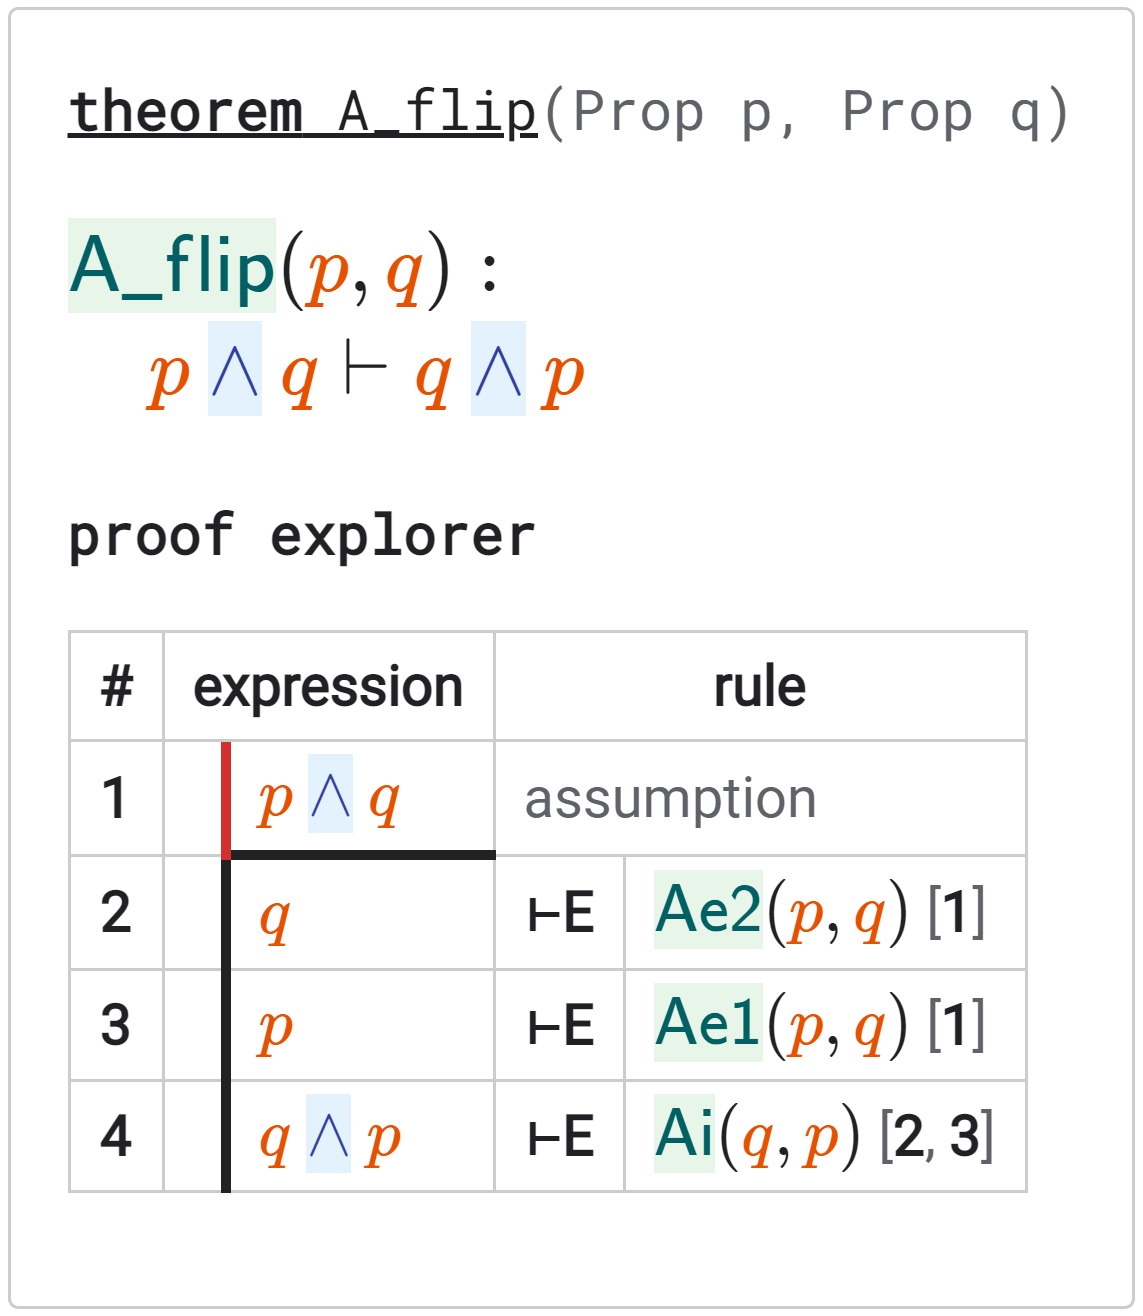
\includegraphics[scale=.18]{A_flip}
	\caption{\texttt{A\_flip}의 증명} \label{fig:Aflip}
\end{figure}


\section{수학의 전산화}

우리는 \texttt{math-o-matic} 체계 상에서 Morse--Kelley 집합론을 기반으로 하여 이항관계, 함수, 자연수 집합 및 정수 집합에 관한 개념을 정의하고 관련 정리들을 증명할 수 있었으며, 이들은 \texttt{math-o-matic} 메인 페이지에서 확인할 수 있다.

\subsection{공리계}

현재 17개의 공리가 정의되어 있으며, 명제논리를 위한 공리계는 예시~\ref{example:system}의 $\Gamma_0$와 같다. 또 술어논리를 위한 공리는 다음의 두 개 뿐이다.
\begin{align*}
	(f^\Predicate)&\mapsto (f\vdash\forall f), \\
	(f^\Predicate, x^\Cls)&\mapsto (\forall f\vdash f(x)).
\end{align*}
$\forall$은 타입이 $\Predicate\to\Prop$인 무정의용어로 정의되는데, 이는 $(\forall x)(f(x))$를 $\forall(x\mapsto f(x))$라고 생각한 것이다. 이외의 공리는 모두 Morse--Kelley 집합론의 공리를 가져온 것이다.

\subsection{증명된 정리들}

다음을 포함한 500개 가량의 정리가 증명되었다.

\begin{itemize}
	\item $1+1=2$.
	\item 수학적 귀납법.
	\item Cantor의 정리.
	\item Schr\"oder--Bernstein 정리.
\end{itemize}

\section{결론 및 향후 연구}

Schr\"oder--Bernstein 정리의 증명은 Fitch 다이어그램으로 300줄 가량인데 나열되어 있을 뿐이라 알기 쉽지 않다.

지금은 체계 $\langle\mathbb A, \mathcal C, \Gamma_0\rangle$을 하나만 만들 수 있으나 여러 개 만들 수 있도록 할 수 있을 것이다. 그러면 공리계 간의 준동형 사상을 생각해 볼 수 있을 것이다. 예를 들어 집합론 상에서의 어떤 집합을 써서 페아노 공리계의 공리들을 증명해 볼 수 있을 것이다.

증명 과정의 자동화도 해볼 수 있을 것이다.

\bibliography{bib}

\end{document}